\documentclass{article}

\usepackage{graphicx}
\usepackage{tikz}
\usepackage{tikzsymbols}
\usetikzlibrary{calc,patterns,shapes.geometric}
\pagestyle{empty}
\usepackage[margin=0pt]{geometry}
\geometry{papersize={14in,12in}}

\def\centerarc[#1](#2)(#3:#4:#5){\draw[#1] ($(#2)+({#5*cos(#3)},{#5*sin(#3)})$) arc (#3:#4:#5);}

\begin{document}
	\begin{figure}
		\centering
		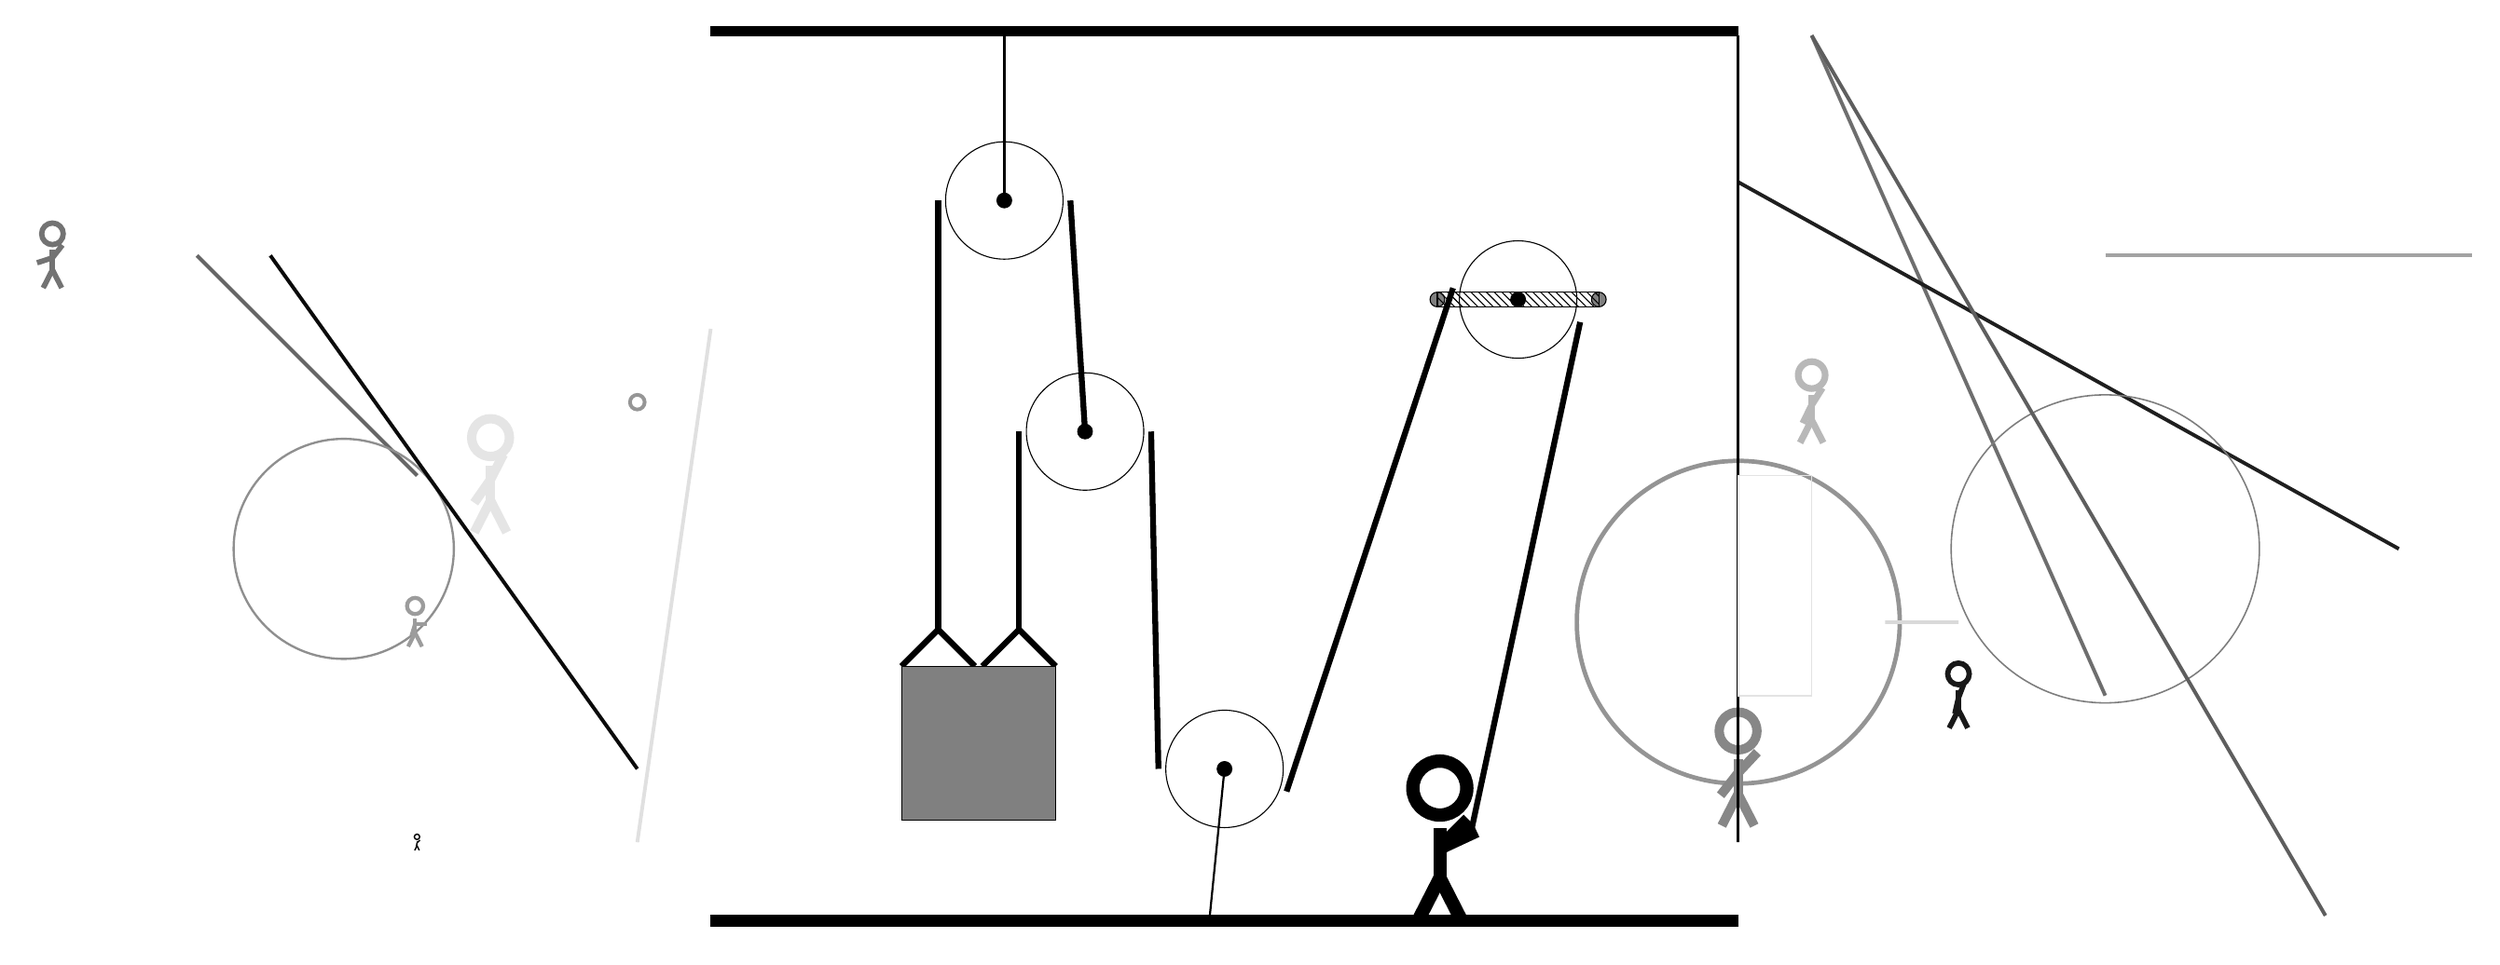
\begin{tikzpicture}
			%%%%% START %%%%%
			
			\draw[fill=black] (-2, 9) rectangle (12, 9.125);
			
			\draw (2, 6.75) circle (0.8);
			\draw[fill=black] (2, 6.75) circle (0.1);
			\draw[thick] (2, 6.75) -- (2, 9);
			
			\draw (3.1, 3.6) circle (0.8);
			\draw[fill=black] (3.1, 3.6) circle (0.1);
			
			\node[line width=0.6mm, color=black!90] at (15, 0) {\Strichmaxerl[4][77][69]};
			
			\draw [line width=0.5mm, color=black!41](-3, 4) circle (0.1);
			\draw[line width=0.5mm, color=black!57](17, 0) -- (13, 9);
			\draw [line width=0.6mm, color=black!42](12, 1) circle (2.2);
			
			\draw[line width=0.5mm, color=black!88](12, 7) -- (21, 2);
			\draw [line width=0.2mm, color=black!51](17, 2) circle (2.1);
			
			\draw[line width=0.5mm, color=black!60](-6, 3) -- (-9, 6);
			\draw [line width=0.3mm, color=black!44](-7, 2) circle (1.5);
			\draw [line width=0.2mm, color=black!85](-10, 2) circle (0.0);
			\node[line width=0.7mm, color=black!99] at (-6, -2) {\Strichmaxerl[1][80][43]};
			\node[line width=0.7mm, color=black!10] at (-5, 3) {\Strichmaxerl[7][55][63]};
			\draw[line width=0.5mm, color=black!63](13, 9) -- (20, -3);
			\draw[line width=0.4mm, color=black!15] (14, 1) rectangle (15, 1);
			\draw[line width=0.5mm, color=black!96](-3, -1) -- (-8, 6);
			\draw[line width=0.5mm, color=black!36](17, 6) -- (22, 6);
			\node[line width=0.2mm, color=black!47] at (12, -1) {\Strichmaxerl[7][52][47]};
			\draw[line width=0.4mm, color=black!99] (12, 9) rectangle (12, -2);
			\draw[line width=0.5mm, color=black!12](-2, 5) -- (-3, -2);
			\node[line width=0.7mm, color=black!55] at (-11, 6) {\Strichmaxerl[4][18][52]};
			
			\node[line width=0.6mm, color=black!28] at (13, 4) {\Strichmaxerl[5][64][58]};
			\draw[line width=0.2mm, color=black!11] (12, 3) rectangle (13, 0);
			
			\node[line width=0.4mm, color=black!39] at (-6, 1) {\Strichmaxerl[3][73][0]};
			
			\draw (5, -1) circle (0.8);
			\draw[fill=black] (5, -1) circle (0.1);
			\draw[thick] (5, -1) -- (4.8, -3);
			
			\draw (9, 5.4) circle (0.8);
			\draw[fill=black] (9, 5.4) circle (0.1);
			\draw[fill=black!50] (7.9, 5.4) circle (0.1);
			\draw[fill=black!50] (10.1, 5.4) circle (0.1);
			\draw[pattern=north west lines, pattern color=black] (7.9, 5.5) rectangle (10.1, 5.3);
			
			\draw[line width = 0.8mm]  (0.6, 0.4) -- (1.1, 0.9) -- (1.6, 0.4);
			\draw[line width = 0.8mm]  (1.7, 0.4) -- (2.2, 0.9) -- (2.7, 0.4);
			\draw[fill=black!50] (0.6, 0.4) rectangle (2.7, -1.7);
			
			\draw[line width = 0.8mm] (1.1, 6.75) -- (1.1, 0.9);
			\centerarc[line width = 0.8mm](2, 6.75)(0:180:0.9);
			\draw[line width = 0.8mm] (2.9, 6.75) -- (3.1, 3.6);
			\draw[line width = 0.8mm] (2.2, 3.6) -- (2.2, 0.9);
			\centerarc[line width = 0.8mm](3.1, 3.6)(0:180:0.9);
			\draw[line width = 0.8mm] (4.0, 3.6) -- (4.1, -1);
			\centerarc[line width = 0.8mm](5, -1)(180:340:0.9);
			\draw[line width=0.8mm](5.8457, -1.3078) -- (8.1137, 5.5562);
			\centerarc[line width = 0.8mm](9, 5.4)(-20:170:0.9);
			\draw[line width=0.8mm](9.8457, 5.0922) --  (8.35, -1.9);
			
			\node at (8, -2) {\Strichmaxerl[10][225][25]};
			
			\draw[fill=black] (-2, -3) rectangle (12, -3.15);
			
			%%%%% END %%%%%
		\end{tikzpicture}
	\end{figure}	
\end{document}